\documentclass{article}
\usepackage[margin=2.5cm]{geometry}
\usepackage{amsmath, amssymb, stmaryrd, latexsym, amsthm, mathtools}
\usepackage{mathpazo, times}
\usepackage{float}
\usepackage{listings}
\usepackage{url}
\usepackage{natbib}
% \usepackage{parskip} % very ugly with lemmas, invariants, etc without intervening text
\usepackage[disable]{todonotes}
\usepackage{slashed}
\usepackage{tikz}
\usepackage{forest}
\usepackage{IEEEtrantools}
\usepackage{microtype}
\usepackage{graphicx,color}
\usepackage{tikz}
\usetikzlibrary{automata, positioning, arrows}
\tikzset{
    state/.style={
           rectangle,
           rounded corners,
           draw=black, very thick,
           minimum height=2em,
           inner sep=2pt,
           text centered,
           },
}

\usepackage{hyperref}
\hypersetup{
  colorlinks=false,
  linkcolor={blue},
  citecolor={blue},
  urlcolor={blue},
  linkbordercolor={white},
  citebordercolor={white},
  urlbordercolor={white}
}
\usepackage[capitalise,noabbrev,nameinlink]{cleveref}

% https://tex.stackexchange.com/questions/132823/ieeetrantools-clash-with-cleveref
\makeatletter
\let\if@IEEEissubequation\iffalse
\makeatother

\newcommand{\coot}[1]{\textcolor{violet}{\emph{#1}}}
\newcommand{\njd}[1]{\textcolor{purple}{\emph{#1}}}
\newcommand{\avieth}[1]{\textcolor{blue}{\emph{#1}}}
\newcommand{\dcoutts}[1]{\textcolor{orange}{\emph{#1}}}
\addtolength{\marginparwidth}{-0.1\marginparwidth}

\newcommand{\var}[1]{\mathit{#1}}
\newcommand{\type}[1]{\mathsf{#1}}
\newcommand{\powerset}[1]{\mathbb{P}(#1)}
\newcommand{\order}[1]{\mathcal{O}\left(#1\right)}
\newcommand{\restrictdom}{\lhd}
\newcommand{\subtractdom}{\mathbin{\slashed{\restrictdom}}}
\newcommand{\restrictrange}{\rhd}

\DeclareMathOperator{\dom}{dom}
\DeclareMathOperator{\range}{range}
\DeclareMathOperator*{\argmin}{arg\,min} % thin space, limits underneath in displays
\DeclareMathOperator*{\minimum}{min}
\DeclareMathOperator*{\maximum}{max}

% Number within sections, and don't have separate counters for separate environments
\theoremstyle{definition}{
  \newtheorem{lemma}{Lemma}[section] % Number within sections
  \newtheorem{definition}[lemma]{Definition}
}
\theoremstyle{theorem}{
  \newtheorem{invariant}[lemma]{Invariant}
  \newtheorem{proofobligation}[lemma]{Proof Obligation}
}

\Crefname{invariant}{Invariant}{Invariants}

\numberwithin{equation}{lemma}

%\floatstyle{boxed}
%\restylefloat{figure}

\lstset{basicstyle=\ttfamily\small}

\raggedbottom

\begin{document}

\title{Design of IPC protocols for Cardano Shelly \\
       {\small (Version 0.7)} \\
       {\large \sc An IOHK technical report}}
\author{Duncan Coutts \\ {\small \texttt{duncan@well-typed.com}} \\
                         {\small \texttt{duncan.coutts@iohk.io}}
   \and Alex Vieth \\ {\small \texttt{alex@well-typed.com}}
   \and Neil Davies \\ {\small \texttt{neil.davies@pnsol.com}} \\
                       {\small \texttt{neil.davies@iohk.io}}
   \and Marcin Szamotulski \\ {\small \texttt{marcin.szamotulski@iohk.io}}
   \and Karl Knutsson \\ {\small \texttt{karl.knutsson@iohk.io}}
   }
\date{November 29, 2018}

\maketitle

\begin{abstract}
This document is intended as a discussion, leading to a design, of IPC
protocols for Cardano's Shelly release. The structure of the discussion is to
look at the requirements and ideas for application-level protocols, before
looking at how those can map onto lower level IPC protocols.

It is a work-in-progress but it is being evolved into a more general document
for the network layer, covering requirements, design and documentation of
lower level protocol details.
\end{abstract}

\tableofcontents

\section*{Version history}

\begin{description}
\item[Version 0.1, June 18, 2018] First draft based on previous notes and
                                  discussions with Alex.
\item[Version 0.2, June 22, 2018] Sketch of protocol proposal and goals for
                                  how to elaborate, based on further review
                                  and discussion with Alex and Neil.
\item[Version 0.3, July 4, 2018]  Comments from Neil.
\item[Version 0.4, July 8, 2018]  New section with alternative broadcast approach by Alex.
\item[Version 0.5, July 13, 2018] Extend the discussion of the alternative broadcast approach.
\item[Version 0.6, July 17, 2018] Fleshed out section on chain following protocols.
\item[Version 0.6.1, July 19, 2018] Minor additional text, to aid understanding.
\item[Version 0.7, November 29, 2018] Consolodated requirements into this document
\end{description}

\section{Introduction}

\subsection{Scope}

This document is intended to cover a number of aspects of the Cardano Shelly
networking system.

It covers the informal high level business requirements. It is intended to
cover the key functional and non-functional requirements, and other technical
and practical constraints

It covers a discussion of the design space within the technical constraints
which is intended to motivate and explain the design choices. It is intended
to be elaborated over time to cover the chosen design. It is also intended
to be extended to document various details needed for interoperability between
implementations: both syntax and semantics.

In understanding the scope of the networking system it is important to
understand that it is not just a local point to point or peer to peer IPC
protocol. It is a distributed IPC facility that has to achieve network-level
outcomes in support of the Ouroboros blockchain distributed application
facility. It must use only local point to point IPC, local knowledge, and
suitable policies together in combination to achieve the network-level
outcomes. It has to achieve this under the constraint of adversarial behaviour
at the network and Ouroboros protocol levels.

It is also worth noting that it is not a general purpose distributed IPC
facility. It is specifically for supporting the Ouroboros blockchain protocol.
Our analysis of the constraints leads us to the conclusion that we must rely
on features of Ouroboros to be able to achieve the information exchange
requirements in the face of adversarial network level behaviour.

In scope for this discussion is IPC that Cardano nodes engage in. We do want
to consider IPC between Cardano nodes and components such as wallets and
explorers, but not between wallets/explorers and other components.

Part of the discussion will be motivated by algorithms, data structures and
resource constraints within nodes, such has how nodes can represent their
blockchains, but this document is not primarily an analysis of those issues.

There are two relatively clearly distinct use cases for IPC for Cardano nodes:
\begin{itemize}
\item IPC between Cardano nodes that are engaged in the high level Ouroboros
      blockchain consensus protocol.
\item IPC between a Cardano node and a `chain consumer' component such as a
      wallet, explorer or other custom application.
\end{itemize}

It is plausible that both use cases could be served by the same protocol, but
this is not a given a priori.

\subsection{Key references}

We will refer both to the original `Ouroboros classic' \citep{ouroboros-classic}
and to the later version `Ouroboros genesis' \citep{ouroboros-genesis}. We will
refer simply to `Ouroboros' where distinctions between the versions are
irrelevant.

\subsection{Goals}

First and foremost the protocols need to achieve their information exchange
requirements.

For the node-to-node protocol this is driven by the functional and performance
needs of Ouroboros. The node-to-node protocol is conducted in a P2P environment
with very limited trust between peers. The node-to-node protocol utilises
store-and-forward over selected \emph{bearers} which form the underlying
connectivity graph. A concern in this setting is asymmetric resource consumption
attacks. Ease of implementation is a nice to have, but is subordinate to the
other hard constraints.

A node-to-consumer protocol is intended to support blockchain applications
like wallets and explorers, or Cardano-specific caches or proxies. The setting
here is that a consumer trusts a node (a `chain producer') and just wants to
catch up and keep up with the blockchain of that producer. It is assumed that
a consumer only consumes from one producer (or one of a related set of
producers), so unlike in the node-to-node protocol there is no need to choose
between different available chains. The producer may still not fully trust the
consumer and does not want to be subject to highly asymmetric resource
consumption attacks. In this use case, because of the wider range of
applications that wish to consume the blockchain, having some options that are
easy to implement is more important, even if this involves a trade-off with
performance. That said, there are also use cases where tight integration is
possible and making the most efficient use of resources is more desirable.

\subsection{Why distinguish node-to-consumer}

It is worth discussing briefly why it makes sense to consider a node-to-consumer
protocol distinct from a node-to-node protocol.

There are a number of applications that simply want to consume the blockchain,
but are able to rely on an upstream trusted or semi-trusted Cardano consensus
node. These applications do not need to engage in the full consensus protocol,
and may be happy to delegate the necessary chain validation.

Examples include 3rd party applications that want to observe the blockchain,
examples being business processes triggered by transactions or analytics.  It
may also include certain kinds of light client that wish to follow the
blockchain but not do full validation.

Once one considers a node-to-consumer protocol as a first class citizen then it
opens up opportunities for different system architecture choices. The
architecture of the original Cardano Mainnet release was entirely homogeneous:
every node behaved the same, each trusted nothing but itself and paid the full
networking and processing cost of engaging in the consensus protocol.  In
particular everything was integrated into a single process: the consensus
algorithm itself, serving data to other peers and components such as the wallet
or explorer. If we were to have a robust and efficient node-to-consumer protocol
then we can make many other choices.

With an efficient \emph{local} IPC protocol we can have applications
like wallets and explorers as separate processes. Even for tightly
integrated components it can make sense to run them in separate OS
processes and the associated OS mamagement tools. Not only is the
timing constraints for a consensus node are much easier to manage when
it does not have to share CPU resources with chain consumers, but it
enables the use of operating system features to give finer control
over resource consumption for sophisticated end-users.  There have
been cases in production where a highly loaded wallet component takes
more than its allowed allocation of CPU resources and causes the local
node to miss its deadlines.  By giving a consensus node a dedicated
CPU core it becomes more plausible to provide the necessary hard real
time guarantees. In addition, scaling on multi-core machines is
significantly easier with multiple OS processes than with a
multi-threaded OS process with a shared-heap. This could allow for
larger capacity Cardano relay deployments where there are multiple
network facing proxy processes that all get their chain from a single
local consensus node.

With an efficient \emph{network} IPC protocol we can do similar things
but extend it across multiple machines. This permits: large
organisations to achieve better alignment with their security
policies; clusters of relays operated by a single organisation to use
the more efficient (less resource costly) node-to-consumer protocol
instead of the node-to-node protocol; Similarly it allows for wallet
or explorer-like applications that need to scale out, and are able to
make use of a trusted node.

\section{Requirements}

\subsection{High level requirements}

These are the high level business requirements for the networking that were
gathered and signed off in late 2017. As such they are expressed in an informal
prose style, and often following a ``user story'' style.

\subsubsection{Network connectivity}

\paragraph{Participate as a user who has delegated}

As a Daedalus home user with my stake delegated to other users I would like to
join the Cardano network so I can participate in the network.
\begin{itemize}
\item The system be designed to provide this user segment with the ability
      catch up and keep up with the blockchain without having to do any local
      network configuration.
\item The system be designed to provide this user segment with the ability to
      continuously find and maintain a discovery of a sufficient number of
      other network participants that have reasonable connectivity.
\item The system be designed to provide this user segment with the ability to
      find and maintain a minimum of 3 other network participants to maintain
      connectivity with performance that is sufficient to catch up with the
      blockchain.
\item The system design will take into account that this user will probably be
      behind a firewall.
\item Users in the segment can be defined by as having all their stake
      delegated to other network participants.
\end{itemize}


\paragraph{Participate in network as small stakeholder}

As a Deadalus home user operating a core node with a small stake, I would like
to join the Cardano network so I can participate in the network as a core node
that produces blocks i.e. have not delegated to someone else.

\begin{itemize}
\item The system be designed to provide this user segment with the ability to
      receive the transactions that will be incorporated into blocks (although
      sizing the operation of the distributed system to ensure that all such
      participants would be able to receive all transactions is not a bounding
      constraint)
\item The system be designed to provide this user segment with the ability to
      participate in the MPC protocol\footnote{This requirement is now
      redundant because the MPC protocol is specific to Ouroboros Classic.}.
\item The system will be designed to provide this user segment with the ability
      to catch up and keep up with the blockchain without having to do any local
      network configuration (this is a bounding constraint).
\item The user will have sufficient connectivity and performance to receive a
      block within a time slot {\sc and} they have to be able to create and
      broadcast a block within a time slot in which the block is received by
      other core nodes.
\item The system will be designed to maximise the likelihood that 50\% of home
      users operating a core node are compliant with the previous requirement
      at any one time.
\item The system will be designed to provide this user segment with the ability
      to continuously find and maintain a discovery of a sufficient number of
      other network participants that have reasonable connectivity.
\item The system will provide a discovery mechanism that will find and maintain
      a minimum of 3 other network participants to maintain connectivity with
      performance that is sufficient to catch up with the blockchain.
\item The system design will take into account that this user may be behind a
      firewall (i.e being behind a firewall should not preclude a user
      participating in this fashion).
\item The Delegation workstream will provide a UI feature for the user to
      choose to control their own stake.
\item Users in this segment will be defined as {\sc not}
      \begin{itemize}
      \item[a)] being in the top 100 users ranked by stake or
      \item[b)] in a ranked set of users who combined control 80\% of the stake
      \end{itemize}
\item Users in this segment will not be part of the Core Diff, but still
      subject to the normal incentives related to creating blocks.
\end{itemize}


\paragraph{Participate in network as a large stakeholder}

As a user running a core node on a server and with large stake in the network,
I would like to join the Cardano network so I can participate in the network as
a core server node that produces blocks i.e. have not delegated to someone else.

\begin{itemize}
\item A large stakeholder will be defined as
      \begin{itemize}
      \item[a)] being in the top 100 users ranked by stake; or
      \item[b)] in a ranked set of users who combined control 80\% of the stake
      \end{itemize}
\item Assuming that this user has sufficient connectivity and performance, the
      system should ensure that the collective operation of the distributed
      system will ensure that they have a high probability, of receiving a
      block within a time slot such that they have sufficient time to be able
      to create and broadcast a block within a time slot where the block is
      received by other core nodes.
\item It is expected that the previous requirement will be fulfilled to a high
      degree of reliability between nodes in this category -- assuming normal
      network operations

      \begin{tabular}{rl}
      Threshold & $>95\%$ \\
      Target    & $>98\%$ \\
      Stretch   & $>99\%$ 
      \end{tabular}
\item The system will be designed to provide this user segment with the ability
      continuously find and maintain a discovery of a sufficient number of
      other network participants that have reasonable connectivity.
\item Discovery will find and maintain a minimum of 10 other network
      participants to maintain connectivity with performance that is sufficient
      to catch up with the blockchain.
\item Ability to receive the transactions that will be incorporated into blocks.
\item Ability to participate in the MPC protocol\footnote{This requirement is
      now redundant because the MPC protocol is specific to Ouroboros Classic.}
\item The user will catch up and keep up with the blockchain.
\item The server firewall rules will be such that it can communicate with other
      core nodes on the system (and vice versa) -- The system will provide the
      necessary information to update firewall rules if the server is operating
      behind a firewall to ensure the server can communicate with other core
      nodes.
\item The threshold which defines the group of large stakeholders may be
      configurable on the network layer. The configuration may include toggling
      between the rules a) and b) in the previous requirement and the threshold
      numbers within these (this is pending a decision from the Incentives
      workstream.
\item The rules and threshold configuration may need to be a protocol parameter
      that is updated by the update system.
\end{itemize}


\paragraph{Poor network connectivity notification}

As a home user, I want to see a network connection status on Daedalus so that
I know the state of my network connection.
%
\begin{itemize}
\item If the user receives a notification that they in red or amber mode,
      Daedalus will give the user some helpful information on how to resolve
      common connectivity issues.
\end{itemize}
%
There are three (at least) distinct modes that the network can be operating in:
each one has a red, green, amber status.

%
\begin{center}
\begin{tabular}{ll}
Initial block sync \\
\hline
red   & receiving $<1$ blocks per 10s \\
amber & receiving $<10$ blocks per 10s \\
green & otherwise  \\[1em]

Recovery \\
\hline
red   & receiving $<1$ slot block per 10s \\
amber & otherwise  \\
green & (not applicable) \\[1em]

Block chain following \\
\hline
red   & it has been more that 200s since a slot indication was received. \\
amber & it has been more than 60s since a slot indiction was received. \\
green & otherwise. 
\end{tabular}
\end{center}

This assumes that the slot time remains 20 seconds.


\subsubsection{Distributed System Performance}

\paragraph{Transaction Throughput}

The transaction per second of the system as a whole will be:
%
\begin{center}
\begin{tabular}{lr}
Threshold &  8 tps  \\
Target    & 16 tps  \\
Stretch   & 50 tps  \\
\end{tabular}
\end{center}

This assumes that the slot time remains 20 seconds.

\paragraph{Transaction Latency}

As a user I want my transaction to be submitted to the blockchain and received
by the target user within the following time period:
%
\begin{center}
\begin{tabular}{lr}
Threshold & 100 seconds \\
Target    & 60 seconds  \\
Stretch   & 30 seconds  \\
\end{tabular}
\end{center}
%
The above time-frames will be achieved for $>95\%$ of all transactions

\paragraph{Network Bearer Resource Use -- end user control}

As a user operating on the network as a home user not behind a firewall, I
would like a cap on the total amount of network capacity in terms of short-term
bandwidth that other network users can request from my connection so I am
assured my network resource is not eaten up by the data diffusion function.

\begin{itemize}
\item The cap should be based on a fraction of a typical home internet
      connection -- it can be changed by configuration including ``don't act
      as a super node''.
\item The system will allow users synching with the latest version of the
      blockchain to download blocks from more then one and up to five network
      peers concurrently.
\item A cap on no. of incoming subscribers.
\item A cap on number of outbound requests for block syncing from other users.
\item The cap will not be imposed on core nodes running on a server.
\item If these resources are available, a reasonable connection speed should be
      available to users requesting to sync the latest version of the
      blockchain e.g. downloading blocks from 5 peers concurrently to aggregate
      the bandwidth.
\item (nice to have) the actual number and capacity being used is available to
      user.
\end{itemize}

\paragraph{Participant performance measurement}

There may be a requirement for measuring if a large stakeholder is not meeting
their network obligation.

It is accepted that this requirement is a ``nice to have'', and it has not been
established that it is possible, nor has it been incorporated into the
incentives mechanism.

\subsubsection{Distributed System Resilience and Security}

\paragraph{Resilience to abuse}

As a user I should not be able to attack the system using an asymmetric denial
of service attack that will deplete network resources from other users.

\begin{itemize}
\item The system should achieve its connectivity and performance requirements
      even in the presence of a non-trivial proportion of bad actors on the
      network.
\item There is an assumption that there are not a large numbers of bad actors
      in the network.
\item The previous assumption does not follow from the assumptions of Ouroboros
      which states that the users that control 50\% of the stake are
      non-adversarial.
\end{itemize}


\paragraph{DDoS protection}

As a large stakeholder running a core node on a server, I should still be able
to communicate with other user in this segment, even if the system comes under
a DDoS attack.

\begin{itemize}
\item Users in this segment will be able to generate and broadcast blocks to
      each other within the usual timing constraints in this situation.
\end{itemize}

IP addresses will be hidden

\begin{itemize}
\item Encrypted IP addresses will be published by 10 of the other members of
      the group of large stakeholder core nodes.
\end{itemize}

Assumption

\begin{itemize}
\item Core node operators will not publish their IP addresses publicly.
\item Encrypted IP addresses will be published by the 10 of the other members
      of the group of large stakeholder core nodes.
\item If a node operators IP address is compromised the operator will respond
      and change the IP address of their node.
\item The system will allow operators to change the address of their core nodes
      and communicate with that new IP address within a reasonable period of
      time.
\end{itemize}


\subsubsection{Network decentralization}

\paragraph{No hegemony}

As a user I want to be assured that IOHK and its business partners are not in
an especially privileged position in terms of trust, responsibility and
necessity to the network so that network hegemony is avoided.

\begin{itemize}
\item IOHK should be in the same position on the network as any other
      stakeholder with an equivalent amount of stake.
\item There is more general requirement that no other actor could do this
      either.
\end{itemize}


\section{Node-to-consumer protocols}

TODO: cover notes on:
\begin{itemize}
\item chain producer representations and in-memory storage with high degrees of forking
  \begin{itemize}
  \item bounds on likely forking numbers, thus bounding the attack surface,
    likely to susceptible to analysis via some (pretty simple - i.e have
    analytical solutions) Markov Chain models.
    \item use-cases
  \end{itemize}
\item chain producer keeping state about consumers
\item immutable vs volatile distinction in representation and protocols
\item stateful protocol
\item stateless protocol
\item recursion as an indicator of completeness \marginpar{\njd{what does this mean Duncan?}}
\item family of protocol variations for different environments: STM, IO, local
  IPC, remote IPC
  \njd{\\noting different levels of implict trust here - we need
    to think whether the STM enviroment is one we treat differently (e.g. trust
    forwarding only correctly signed blocks reducing the checks in the consumer
    end) or do we assume even shared process nodes are potentially missbehaving
    and play up the way in which that helps defend against other forms of attack? }
\item optimised case for immutable chain, e.g. shared files
\item STM interface
\item coping with talking to a load-balanced cluster of imperfectly synced producers
\end{itemize}

\subsection{Goals}

\paragraph{Family of protocols}
We are interested in a family of chain following protocols to cover a range of
use cases. We are interested in:
\begin{itemize}
\item in-process protocols to be used for in-process chain consumers and as an
      aid to implementing the producer side of inter-process protocols.
      These will likely be exposed as APIs using STM or IO.
\item OS-local IPC protocols for out-of-process chain consumers
      such as wallets, and for implementing and scaling out the producer side
      of IPC network protocols.
\item efficient network IPC protocols for remote chain consumers, including
      wallets and network relays or proxies.
\item convenient stateless network IPC protocols for remote chain consumers
      where a trade-off towards the convenience of consumer implementation is
      appropriate.
\end{itemize}

In all these cases we will refer to the protocol peers as the chain producer
and the chain consumer or follower.

\paragraph{Recursion as an indicator of completeness} As mentioned, part of the
intention of having a family of related protocols is to be able to use some to
help implement others, but also to chain combinations together to allow
flexibility in application design. A measure of the completeness of each
protocol family member is that the consumer side should be enough to implement
the producer side of the same protocol or of another protocol in the family
(e.g. the consumer side of an in-process protocol being sufficient to implement
the producer side of one of IPC protocols).
\njd{I don't quite get this - are you implying some sort of `protocol duality' here?}

\paragraph{Resource use with misbehaving peers}
In the IPC cases we are interested in protocols where the chain producer can
ensure reasonable resource use even when the peer misbehaves to some degree. In
particular we do not want slow consumers to force excessive resource use by the
producer.

\paragraph{Consistent resource use}
In a system such as Cardano that has timing constraints and is operated by many
different users, there is a concern about the \emph{consistency} and
\emph{predictability} of resource use. As an example, if a process in the system
typically uses a certain amount of memory then operators who deploy that
process will tend to provision the host system's resources to accommodate that
typical memory requirements and will not provision too much extra memory (as
that would cost more). If the process has quite different memory requirements in
a worst case vs a typical scenario then this potentially constructs a serious
hazard: if the worst case scenario can be forced by adversaries then this
provides a mechanism for adversaries to cause resource exhaustion and denial
of service on very many nodes in the system simultaneously -- perhaps enabling
further attacks once many honest nodes are offline.

Even if the worst case resource requirements are clearly documented for
operators it is inevitable that resources will not be reserved: operators will
ignore the documentation, or automatic systems will reclaim unused resources
and not be able to provide them in time when they are needed. The practice of
manual or automatic `thin' provisioning exacerbates the issue.

The best solution is, as far as possible, to use the same amount of resources --
such as memory -- at all times. This means selecting and designing algorithms
to avoid significant differences in resource consumption between worst case and
best case situations. This may mean forgoing opportunities to reduce resource
use in benign situations to maintain consistency across all situations.

Even if the resource use is not attacker controlled, it is good to avoid
`spikey' resource use for similar reasons, especially if the spikes are
synchronised between instances\footnote{In the current implementation epoch
boundaries are a good example of synchronised resource spikes.}.

\subsection{Forking and resource bounds}

A chain producer following the Ouroboros protocol (or following another chain
producer) can of course switch forks and hence chain following protocols must
support this, and support it with reasonable resource bounds.

In Ouroboros Classic there is a helpful constraint that the maximum length an
alternative fork can diverge from the current chain is $K$ blocks. Ouroboros
Genesis does not need this constant but it appears that it could be
reintroduced without too much difficulty.

The benefit of this constraint is that it divides the blockchain into
two parts: a genuinely \emph{immutable} initial chain and a
\emph{volatile} recent chain fragment. An immutable chain allows
implementation options with simple and efficient on-disk storage for
the chain representation and other associated data structures. A
volatile fragment that is bounded in length allows implementation
options using combinations of in-memory and on-disk data storage.  In
particular, keeping track of up to $K$ blocks can easily be
accommodated in memory\footnote{The current implementation uses
  $K = 2160$.}.

Figure \ref{chain-diagram-imm-vol} illustrates a representation comprised of
immutable and volatile parts. Incidentally, it illustrates a couple possible
design choices: to have significant overlap between the immutable and volatile
parts, and for the immutable part to trail somewhat behind the most recent K
blocks.

\begin{figure}
\pgfdeclareimage[height=3cm]{chain-diagram-imm-vol}{chain-diagram-imm-vol.pdf}
\begin{center}
\pgfuseimage{chain-diagram-imm-vol}
\end{center}
\caption{A blockchain representation comprised of immutable and volatile parts.}
\label{chain-diagram-imm-vol}
\end{figure}

While the volatile chain fragment is only $K$ long, a chain following protocol
has to help chain consumers follow the volatile part of the chain as it
switches between forks and this may need to store more information.

Two general approaches to chain following protocols are as follows:
\begin{itemize}
\item The consumer and producer maintain enough information so that on a fork
      the producer and consumer are able to immediately and precisely determine
      how far the consumer has to roll back their chain before rolling forward
      on the new chain.
\item On a fork the consumer and producer have to engage in a protocol to
      determine where (roughly or precisely) the intersection between the
      consumer and producer's chains is and thus where the consumer needs to
      roll back to before rolling forward.
\end{itemize}

The first approach leads to more stateful protocols and the second approach to
stateless protocols. An appealing aspect of the first approach is being able to
go directly to the right place without needing any further steps.

A simple design following the first approach would be for the producer to keep
track of all forks it has gone through, at least within the last $K$ blocks.
This provides enough information for the producer to know the exact relationship
between old forks and the current chain, so that any consumer on any old fork
could be informed how to move to the new fork. The problem with this design is
that it could in the worst cases involve keeping track of a lot of forks, up to
$\mathbf{O}(K^2)$ of them. If we keep them all in memory then this would set up
exactly the kind of attacker-controlled resource spike that we are trying to
avoid. If we keep them all on disk then we lose the simplicity of an in-memory
design.

A plausible alternative design involves the producer not keeping track of all
old forks, but instead keeping track of all the chain consumers and what old
forks they were on. In this design, instead of needing memory proportional to
the number of possible forks, it needs memory proportional to the number of
consumers. In particular it is possible to keep track of just the last $K$
blocks in the chain and $\mathbf{O}(1)$ state per consumer, giving an overall
complexity of $\mathbf{O}(K + C)$ for $C$ consumers. It is of course expected
that the number of consumers will be limited according to available resources.

\subsection{Sketch of a stateful chain following IPC protocol}
\label{sec:stateful-ipc}

In this stateful protocol there is a communication session with a bidirectional
unicast channel between the chain producer and chain consumer. It is stateful
in the sense that the chain producer maintains some state about the state of
the chain consumer. The state that the producer maintains about the consumer
is the `read pointer'. This tracks what the producer knows about the head of
the consumer's chain.

\begin{figure}
\pgfdeclareimage[height=6cm]{chain-diagram-read-pointers}{chain-diagram-read-pointers.pdf}
\begin{center}
\pgfuseimage{chain-diagram-read-pointers}
\end{center}
\caption{Representation of a producer's chain, including `read pointers' for two example consumers.}
\label{chain-diagram-read-pointers}
\end{figure}

Figure \ref{chain-diagram-read-pointers} illustrates an example producer's
chain plus tracking for two consumers. In the example, consumer A illustrates a
typical case where the consumer's read pointer is on the producer's chain,
while consumer B illustrates a case involving a fork. We will elaborate both
cases.

\paragraph{Request/Response interaction}
The form of interaction between the consumer and producer follows a simple
request/response pattern driven by the consumer. The consumer makes a request
to ask for the next state change and the producer replies with an instruction
on how the consumer should change its state. These update are either to roll
forward to a given block (supplied by value or by reference), or to roll
backwards to a given point on the client's chain.

The consumer-driven pattern effectively flips round to being producer driven in
the case that a consumer is at the head of the producer's chain. In this case
the consumer issues the request but the producer does not reply until the
producer's own chain state changes (by adding a new block or switching fork).
So in this state the consumer is waiting and it is the producer that will
initiate the next change by pushing an update to the consumer. So it is
still the same request/response pattern, but with a long delay before the
response.

The protocol is agnostic about whether it is just block headers or full blocks,
and it is agnostic about whether blocks are provided by value or by reference.
The protocol can be instantiated with any choice of these details.

\paragraph{Typical case: consumer on the current chain}
In the typical case (consumer A in Figure \ref{chain-diagram-read-pointers}),
the read pointer is on the producer's chain and is not yet at the chain head
so there is a next block. In this case when the consumer requests the next
instruction, the producer simply sends the next block. \marginpar{\coot{It's probably more
efficient to subscribe for updates, and the producer could just push
instructions, but maybe this does not matter at this level of description.}} The
producer can assume that the consumer will update its local state and so the
producer can update the read pointer to point to the next
block.

\paragraph{Producer state change: adding a block}

As mentioned above, if the read pointer is at the head block when the consumer
asks for the next instruction then the producer's response is delayed until
the producer's own chain next changes. When the producer's state changes by
adding a block then all consumers that were at the chain head and are waiting
on a response will be sent a response containing the new block.

\paragraph{Interesting case: consumer on an old fork}
The more interesting case is the case involving forks. In the example of
consumer B in Figure \ref{chain-diagram-read-pointers}, the consumer was at
block 41, hash 0x660f, which is on an old fork that is no longer on the
producer's chain. The state that the producer has in this case records the fact
that the consumer was at this old block, but the read pointer points to the
location on the producer's chain that the consumer will need to move to. So
when the consumer asks for an update the producer will send an instruction to
tell it to rollback to the given block. The producer will then update its read
pointer to record the fact that the consumer is now back on the chain at the
target block (39, hash fa40 in the example).

So it is clear that the producer's state about the consumer has two cases, the
normal case and the fork case. In the fork case the location of the read
pointer is at the target block on the current chain to roll back to.

\paragraph{Producer state change: switching fork}

The situation when a read pointer state gets into the fork case is when the
producer's chain switches fork. A fork switch involves removing some number
of recent blocks and adding more blocks. The producer must update any consumer
read pointers that point to the blocks that are being removed. The recorded
state must remember the block that the consumer was at, but the read pointer
must move to the block that the consumer will be asked to roll back to.

It is worth pointing out here is what happens for read pointers that are
encountered when removing block that were \emph{already} in the fork state.
The read pointer is simply moved as normal, and the original state recording
which block the consumer was at is preserved. This explains why the read
pointer for the fork state has to be at the block on the current chain that the
consumer will roll back to rather than at the block on the old fork: it is so
that if there is a further fork the read pointer can easily be found and moved.

\coot{
    Let's analyze what will happen when a consumer is following more than one
    producer in a subscription model rather than request / respond model.  It
    may happen that the consumer will receive two different instructions.  Let
    say that producer $p_1$ and producer $p_2$ are pushing the consumer to
    switch to two different blocks that follows consumers tip (a fork happens).  The
    consumer will solve a tie and choose one of the forks, let say $p_1$'s
    fork.  The producer $p_1$ does not need to be informed about the tip
    change of the consumer.   When $p_1$ will build on top of his fork he will
    send instructions to rollback and follow to his tip and if his chain will
    loose he will have a way to inform the consumer how to proceed.  It seems
    that we need the following two invariants:
    \begin{itemize}
    \item the producer knows how to connect his tip with read pointer of the
        consumer
    \item the consumer should not delete the header at which producer's read pointer points to
    \end{itemize}
    Furthermore, together with a rollback - roll forward instruction from
    a producer, the consumer should get the height of the chain from the
    read pointer to producer's tip.  This can be used to choose which producer
    to follow, in case of multiple choices from different producers.  This is
    just an optimisation for resource usage (bandwidth and memory usage).
    This message should be validated if it does not extends a chain to the
    future.  This simple measure can save resources that would be wasted
    downloading and validating headers.
}

\paragraph{Establishing a new consumer session}

So far we have covered the operation once a session is established. To
establish a new session we must establish the read pointer state for the
consumer on the producer side. This involves finding the intersection between
the producer and consumer's chains, sometimes called the \emph{last common
ancestor} (LCA).

The consumer opens by sending a list of points on their chain. These points
are pairs of slot number and block hash. The list is in order of the slot
number. There is some flexibility in which points the consumer sends but it
must include the head block and -- to guarantee that an intersection can be
found -- the block K back from the head. This guarantee is so because the
longest fork the producer could have had is K blocks and so provided the
consumer was previously following the same producer's chain then the block K
back is guaranteed to still be on the producer's current chain.

A reasonable choice for a list of points is be the consumer's current chain
head and then points $\{2^n ~ | ~ n \in \{1\ldots\},  2^n \leq K\}$ earlier.
The producer can compare these points with its own chain to find the first
point that is on its chain. This gives a range in which the intersection point
is known to be. The producer establishes the initial read pointer as follows.
\begin{itemize}
\item If the consumer's chain head block is on the producer's chain then the
      read pointer is established in the normal state, pointing to that block.
\item If the consumer's chain head block is \emph{not} on the producer's chain
      then the read pointer is established in the fork state recording the
      consumer's head block and pointing to the block at the older end of the
      range in which the intersection point is known to be. This state means
      that if the consumer asks for the first update it will be told to roll
      back to (the lower bound on) the intersection point. This is a safe
      approximation but could waste re-sending many blocks.
\end{itemize}
At this stage we have at least established a safe lower bound on the
intersection point and set up a read pointer so that we could proceed with the
main protocol from here. The only remaining problem is one of efficiency if
the range for the intersection point is large. So at this stage there are two
cases depending on the size of the range for the intersection point.
\begin{itemize}
\item If the size of the range is below some agreed threshold then we are
      essentially done: the read pointer is established and the producer can
      reply informing the consumer that this is now the case.
\item If the size of the range is above the threshold then we need further
      steps to narrow down the range.
\end{itemize}
In the latter case the further steps are as follows. The producer has already
established the read pointer at the older end of the range. It now sends back
the block range and an ordered list of points from its chain that fall within
the range. Again these points are pairs of slot number and block hash. A good
choice of points are ones that divide the range into sub-ranges of almost equal
size.

The consumer now inspects these points from the producer and determines which
ones occur on its chain, thus narrowing down the range in which the
intersection point must fall. The consumer may now send a further list of
points within the range it has determined. The producer uses these points to
`improve' the read pointer by moving it forward if possible. This is done by
checking which if any occur on the producer's chain. If the producer's chain
has switched fork since the producer sent its initial response then it may be
the case that none of the points the consumer sends do occur on the producer's
chain. In this unlikely case the read pointer is not altered and no improvement
is made.

\dcoutts{Does it make sense to generalise this slightly and allow the
`improvement' message at any time? All it does is optionally improve the read
pointer on the producer side. Are there ever cases where it'd be useful beyond
the initial establishing of the session?}

\subsection{Sketch of a stateless chain following IPC protocol}



\section{Node-to-node protocol}

The Ouroboros consensus protocol \citep{ouroboros-classic, ouroboros-genesis}
describes what it needs from its network layer. Informally, that:
\begin{itemize}
\item nodes that create a new block in a time slot need to be able to broadcast
      their \emph{entire blockchain} to all other nodes, and;
\item within each time slot, all nodes to collect \emph{all the blockchains}
      they have received via broadcast and then to pick among them.
\end{itemize}

The challenge is to simulate this specification in bounded resources and to do
so without opening up opportunities for new attacks at the network level. Such
attacks might include preventing broadcast or local denial of service by making
nodes consume excess resources (time, memory, network, CPU).

There are a few aspects to bounding resource use in this setting.
\begin{enumerate}
\item We can try to establish some absolute bound on the required resources.
\item With or without an absolute bound we can try to arrange things so that it
      is difficult for an adversarial party to create a lot of work for honest
      parties.
\item If we cannot establish absolute resource bounds for a perfect simulation,
      or the bounds might be too large for some instances, we can consider what
      choices an instance with limited resources should make to achieve a good
      enough simulation.
\end{enumerate}

Obviously na\"ively broadcasting entire chains is not something that can be
done with bounded resources since there is no bound to the chain length.
Obviously the intention is to communicate new blocks and to share and reuse the
parts of the chain that have not changed, though this is easier said than done.

There is however another dimension to the resource bounding problem. In a
proof-of-work blockchain protocol it is expensive for adversarial parties to
create lots of `fake' blocks, so there is in practice a limit on the number of
such blocks that honest parties need to consider. In proof-of-stake blockchain
protocols there is no such constraint: adversarial parties can create many
signed blocks.

\subsection{Drawbacks in the current Ouroboros network protocol implementation}

In the current architectural deployment there is an assumption that certain
nodes are being run by trusted parties and, as such, non-adversarial. There is
no current formal argument as to how, in the presence of nodes acting
adversarially with respect to data diffusion, at what level of adversarial
action performance is compromised.

It is unclear if or how the chain broadcast logic corresponds to the chain
broadcast specified in the Ouroboros paper. Rather than implementing broadcast
directly, it interleaves chain adoption with relaying of block headers. This
may not be wrong, but there is no stated argument for it being faithful.

The chain broadcast logic is vulnerable to straightforward resource consumption
attacks: it responds to receiving a new chain head header by trying to chase
that down before doing anything else. If this is slow (and attackers can make
it slow) the logic does not proceed with considering headers from any other
peer.

The broadcast and chain logic are intertwined in ways that are complex and
increase latency for relaying blocks, which limits the diameter of the network
that can be supported for a given slot length.

\subsection{Broadcast in the context of chain selection}

The major challenge in the design of a practical IPC protocol for Ouroboros is
to find something that satisfies what Ouroboros specifies but does so in a way
that is not open to various kinds of attacks from adversarial nodes.

Ouroboros specifies the overall state changes involved in agents obtaining
and selecting candidate chains. The specification describes the state changes
in a modular way, composed of two phases: broadcast of chains followed by
selecting amongst all the candidate chains received.

As mentioned previously, broadcasting whole chains is not practical, but it is
relatively straightforward to recast this in in terms of broadcasting (or
relaying) blocks.

The more subtle problem is that while the specification describes chain
broadcast and selection as separate phases, we cannot implement them separately.
We must implement \emph{broadcast in the context of chain selection}, meaning
that we must take advantage of the constraints imposed by chain selection to
limit what can be broadcast. If we provided broadcast directly without any
constraints then it could easily be abused by adversaries to conduct highly
asymmetric resource consumption attacks.

So we want a design that achieves the equivalent effect of chain broadcast
followed by local chain selection, but it is acceptable to intermingle the
chain selection logic with the broadcast logic, indeed it would appear to be
necessary to achieve a design that works in bounded resources.

\subsection{Interleaving chain selection with relaying}

With the previous point in mind, it is tempting to consider pursuing an
approach where each node subscribes to and follows the chains of a number of
its peers and continuously selects between those chains following the Ouroboros
chain selection rule. The intuition is that that this should make it easier
bound a node's resource use since it only need consider the N potential chains
from its N immediate peers.

The challenge in this interleaving approach is that the argument that it is
equivalent to what Ouroboros specifies is not trivial. By contrast the
equivalence argument is much clearer if we broadcast the block header of each
chain's head and then chase down the rest of the chain back to an intersection
point.

\subsection{Basic techniques to help bound resource use}

There are a number of tricks to help bound resource use that are standard for
blockchain communication. We can break up the blockchain into individual blocks,
and blocks themselves into a small fixed size header and a larger variable
sized body. The basic idea is that we initiate a chain broadcast by
communicating the block header for the head block in the chain.

In PoW blockchain algorithms the header can contain the representation of a
proof of work, while in PoS the header contains representation of the proof of
stake: a signature showing that it was created by the appropriate party. In
Ouroboros the PoS signature means that nodes that are up to date (at least
within the same epoch) can verify that the header itself is plausible, and
exclude incorrectly signed or implausible headers.

A small fixed size header means that we can bound the network resource use
to send or receive a single header, and can also bound the CPU resources needed
to verify the header.

\subsection{Review of constraints on chain broadcast}

The Ouroboros algorithm imposes a number of useful constraints on chain
broadcast.

\begin{itemize}
\item Ouroboros specifies that chains with blocks from slots in the future are
      invalid. The signed block header contains the slot number so we can
      exclude such chains just by looking at the block header of the head block
      in the chain (which is the one we broadcast).
      \avieth{If a slot leader can mint a new block and deliver the header to
      a peer within the clock skew of that peer then it may be incorrectly
      rejected. We may want to set some tolerance threshold.}
\item Ouroboros specifies that when a node adopts a new chain it only ever
      picks one strictly longer than its current one. The signed block header
      contains the block number so by comparing the block number of the
      broadcast header against the current length of the node's chain, we can
      exclude chains that are shorter and so could never be picked.
      \avieth{Further, it is never necessary for a node to relay a chain when it
      knows of a better one. This may be very useful in practice: at most one
      chain must be tracked per peer. An adversary cannot make an honest node
      retain multiple chains of its own broadcast.}
\item Ouroboros Classic (but not Genesis) specifies that a node will only ever pick
      a chain that diverges from its current chain within the last K blocks,
      implying that forks can be at most K long. This places a bound (of K) on
      the range in which a node needs to look for an intersection between the
      new purported chain (represented by the header of its head block) and its
      own current chain. This bounds the number of block headers that a node
      would ever need to download to obtain all headers for the candidate chain.
\item Each block must be signed by the appropriate slot leader. This signature
      -- which is the proof of stake -- can be checked by any node that has
      the chain up to the current epoch.
\item In Ouroboros Classic, there is only ever one legitimate leader for each
      time slot, and non-adversarial players never sign more than one block
      for the slots in which they are the leader.
\item In Ouroboros Genesis, the situation is similar: there can be more than one
      legitimate leader for a time slot but the number of leaders in a slot
      follows a distribution that makes a large number highly unlikely (and
      this is not controlled by adversarial players). Again, non-adversarial
      players never sign more than one block for the slots in which they are
      the leader.
\item In both Ouroboros Classic and Genesis it is possible for adversarial
      players to sign multiple blocks for the same slot.
\item \avieth{Theorem 4.13 from the original Ouroboros paper describes the
      probability of the existence of a flat fork of length $n$: 2 tines of
      equal block count intersecting $n$ slots prior. This is applicable to
      what we're doing here, both for resource bounds and for correctness.}
\end{itemize}

\subsection{Discussion of bounds}
\dcoutts{This section needs to be revised in the light of the interleaving
approach.}

The combination of these constraints does place a limit on the number and
length of plausibly valid chains that an adversary can create and try to get
honest parties to chase. Given that some honest parties may have gone offline
and be a long way behind the chain, and in particular will not be able to
validate signatures in block headers. So it is worth splitting the analysis
into the case of nodes that are within the current epoch, and a case for nodes
that are further behind. We start with the first case.

In particular, plausibly valid chains would have to start with a valid header
that falls into a slot after the last block of the target victim's chain
but only up to the current time slot. Plausibly valid chains can only extend
back up to K blocks (max 2K slots). The victim is able to assume that other
honest nodes do not sign more than one block per slot, this imposes the
constraint that the adversary can only send one header per slot within the
range just described.
\avieth{Why? I don't see it. Plausibly valid chains can extend more than
  K blocks, no? Maybe the language is unclear.}

It is worth noting that just because honest nodes do not sign more than one
block per slot, it does not mean that different honest nodes will not have
different blocks in the same slot, since an adversary can in previous slots
have sent different headers to different nodes.

\njd{\centering I'm not certain I agree with this, or perhaps I don't agree
  with the implied generality. Honest generator nodes will only generate one
  block per slot - so only one of those can exist per slot. Dishonest nodes can
  generate many such blocks, agreed - maybe that needs to be brought out.}

\avieth{What's the disagreement here?}

\paragraph{An overall bound} Suppose the victim node has a chain with
at least $K$ blocks covering the last $K \leq s \leq 2K$ slots, and $n$ slots
between the slot of the head block of chain on the victim node's and the
current time slot. Suppose also that the adversary controls a fraction
$0 \leq \rho < 1/2$ of the stake in the current epoch.

In that case the adversary can create approximately $n * \rho$ chains (the
specific slots in which the adversary is leader is drawn from a probability
distribution). In the worst case this approaches $n / 2$, but of course the
adversary is allowed to wait until it gets lucky in the probability
distribution. Each of these chains can be up to approximately $(n+K) * \rho$
long. Of course only the chains that are actually longer than the victim node's
current chain are valid.

\njd{This would seem to be the right spot for the simple MC analysis on
  distribution of burst lengths\\
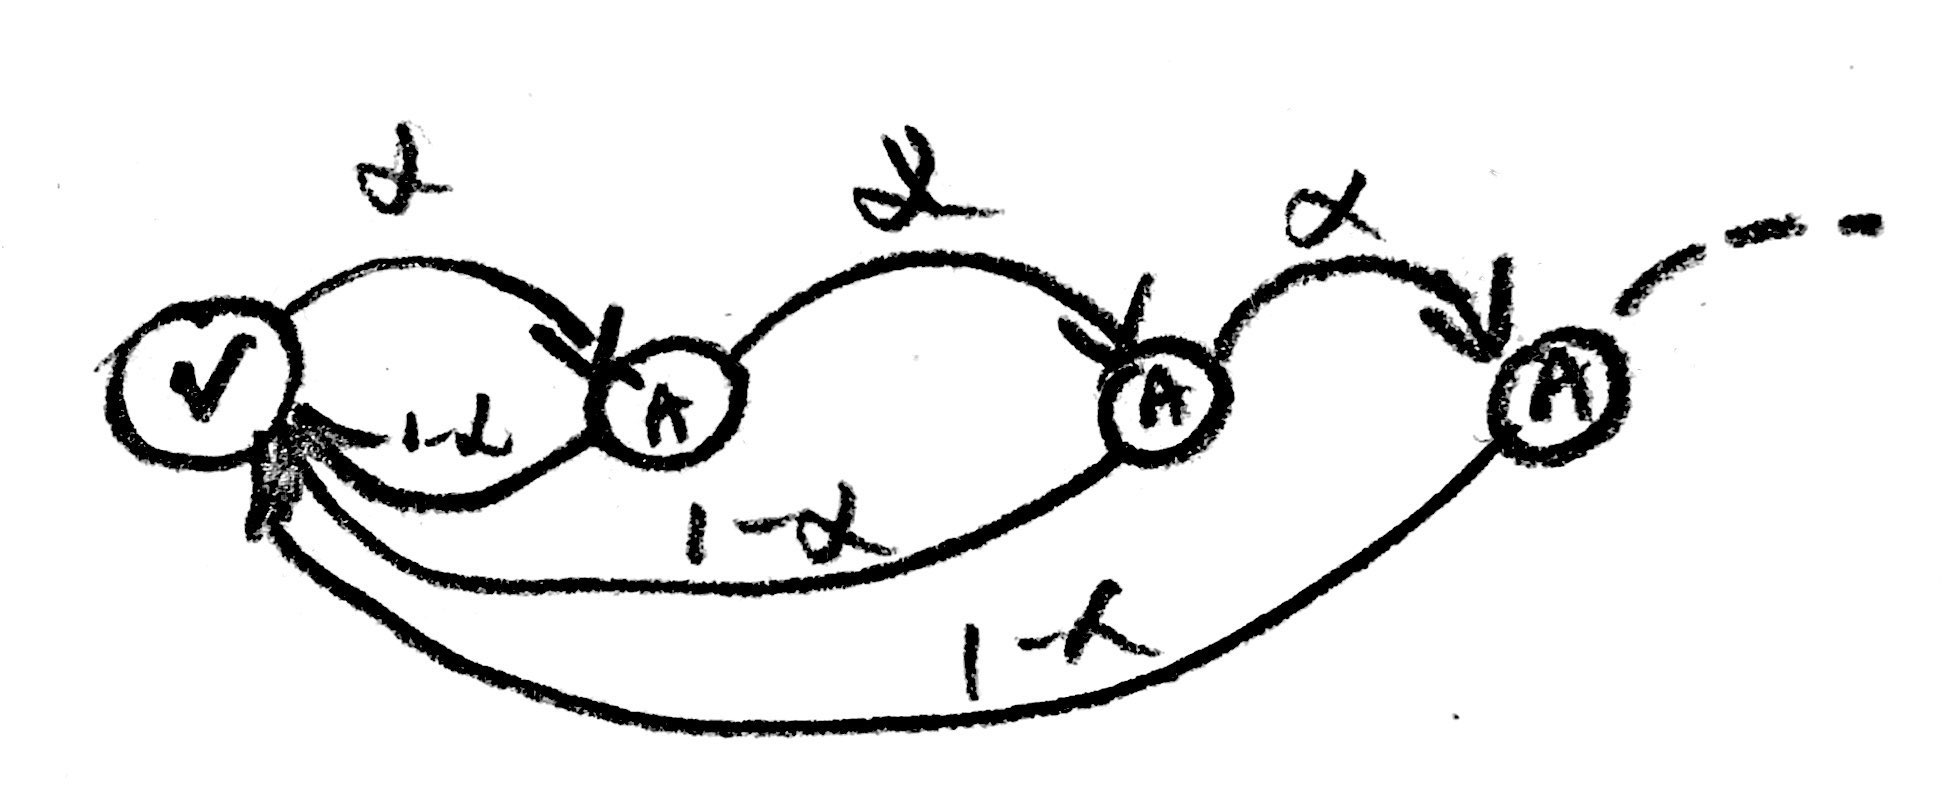
\includegraphics[totalheight=2cm]{burst-length-mc.png}}

\subsection{Plausible design approaches}

As discussed above we must design chain broadcast in the context of chain
selection. There are at least two plausible design approaches that we have
considered.

The first involves relaying the block header of the chain head followed by
chasing other block headers and bodies. It involves taking advantage of the
chain validity and selection rules to apply validation as early as possible,
including checking the signatures on block headers. It does not however involve
intermediate nodes adopting a chain prior to relaying.

The second does involve intermediate nodes adopting a chain prior to relaying.
Each node keeps track of the chains of its immediate neighbours in the network,
which is equivalent to nodes relaying their chains once they have adopted an
updated chain. So a new chain can propagate from node to node but at each
hop it is only relayed if the node selects the new chain itself.

An advantage of the first approach is that it is easier to argue that it is
equivalent to what Ouroboros specifies. By relaying block headers in advance
of requesting blocks and doing full chain validation it is possible to minimise
the hop-by-hop latency.

An advantage of the second approach is that by doing more validation in advance
of relaying, the number of initially plausible but ultimately invalid chains
that each node must consider can be curtailed considerably. The second approach
would appear to involve less implementation complexity by avoiding having to
track the state of multiple outstanding requests for more block headers and
bodies and may be able to reuse much of the implementation of a node-to-consumer
chain following protocol. A disadvantage is that the simplest approach to
adopting a chain before forwarding would involve a high hop-by-hop latency
since a block header could not be sent on before a block body was received.
More complex variants may be able to overcome this limitation. And of course
the whole approach is only legitimate if we can convincingly argue that it is
equivalent to what Ouroboros specifies.

\subsection{An argument for interleaving chain selection with relaying}

This is an attempt to construct an informal argument that designs based on
interleaving chain relaying with chain selection may be equivalent to chain
broadcast followed by chain selection.

Let us start with the basic model: chain broadcast followed by chain selection.
In this model all nodes are able to send on a broadcast channel and all nodes
can reliably receive chains on this channel. The slot leader adds a new block
to its chain and sends it on the broadcast channel to all nodes. In each time
slot, all nodes collect all chains received on the broadcast channel into a set.
At the end of the time slot each node selects their best chain, given their
existing chain and the set of candidate chains received via broadcast. The
chain selection function selects the longest valid chain that is longer than
the current chain. Ties are broken arbitrarily.

An argument that some other proposed model is equivalent to this basic model
has to argue that the chain that is selected by each honest node is the same
as in the basic model. In this context `the same chain' can involve refinements
of the arbitrary choice between chains of the same length. More precisely we
could recast the chain selection function to return the set of all alternatives
which we are indifferent between. In this style we can say that a model is a
refinement if the set of selected alternative chains is a non-empty subset of
the set from the original model.

Let us now consider a model that is one step in the intended direction but
still relatively simple. Instead of a broadcast channel, assume that the
nodes are arranged in a graph with unicast channels on the graph edges. We
assume that all honest nodes are at least connected to each other via other
honest nodes\footnote{This is an assumption that any refinement to a P2P
network needs to make, and an assumption that the P2P connectivity layer must
discharge.}. The slot leader adds a new block to its chain and sends it on the
unicast channels to all its immediate neighbour nodes. Upon receiving a chain
on a channel from a neighbour, a node validates the chain and does chain
selection between the new candidate chain and its current chain. If it selects
the new chain then it relays the new chain on the unicast channels to all its
immediate neighbour nodes.

This model involves switching from chain selection as an operation on a set of
candidate chains and the current chain, to being a binary operation between a
single candidate chain and the current chain. We claim as a lemma that
compositions of the binary operator version is equivalent to the whole-set
version, modulo differences between indifferent alternatives.

\begin{align*}
\mathsf{selectChain} & \in \mathsf{Chain} \to \mathbb{P}~\mathsf{Chain}
                                          \to \mathbb{P}~\mathsf{Chain} \\
\mathsf{selectChain} ~ c ~ cs & = blah
\end{align*}

\coot{\subsubsection{Selection functions}}

\begin{definition}
    \coot{A selection on a set \(A\) is a family of functions
    \(f_n:A^n\rightarrow A\) such that}
    \begin{enumerate}
        \item[F1] \coot{\(f_1:A\rightarrow A\) is an identity function}
        \item[F2]\coot{\(f_n\circ\sigma' = f_n\) for any permutation \(\sigma\),
            where \(\sigma':A^n\rightarrow A^n\) is defined by
            \(\sigma'(a_1,\dots,a_n)=(a_{\sigma(1)},\dots,a_{\sigma(n)})\)}
        \item[F3]\coot{\(f_n(f_{m_1}(a^1_1,\dots,a^1_{m_1}),\dots,f_{m_n}(a^n_1,\dots,a^n_{m_n}))=f_{m_1+\dots+m_n}(a^1_1,\dots,a^m_{m_n})\)}
    \end{enumerate}
\end{definition}

\begin{lemma}
    \coot{There is a bijection between the set of selections on a set \(A\)
    and abelian semigroup multiplications on \(A\) defined by:
    \((f_n)\mapsto f_2\)
    }
\end{lemma}
\begin{proof}
    \coot{
        Given \(g:A^2\rightarrow A\) an abelian semigroup multiplication on
        \(A\) a \(n\)-th
        selection function \(f_n:A^n\rightarrow A\) is defined by
        $$f_n(a_1,\dots,a_n)=g(\dots g(g(a_1,a_2),a_3),\dots,a_n)\ for a_i\in
        A\ \mathrm{and}\ n>1$$
        Furthermore so constructed selection satisfies axioms \rm{F1}, \rm{F2} and
        \rm{F3}.
    }
\end{proof}
\subsection{Sketch of a design for interleaving chain selection with relaying}

We assume a peer discover mechanism that establishes associations between
nodes, from which each node selects and establishes connections with a small
number of peers (on the order of 3-8). The rest of the description will be
from the perspective of a single node within this graph.

The node uses the chain following protocol from Section \ref{sec:stateful-ipc}
with each of its connected peers. It uses this protocol independently for each
peer to give us a \emph{candidate} chain for each peer. At a high level the
idea is that the node's own chain will be continuously selected from the set of
candidate chains by following the normal Ouroboros chain validation and chain
selection rules.

\begin{figure}
\pgfdeclareimage[height=6cm]{node-diagram-chains-state}{node-diagram-chains-state.pdf}
\begin{center}
\pgfuseimage{node-diagram-chains-state}
\end{center}
\caption{Representation of a producer's chain, including `read pointers' for two example consumers.}
\label{node-diagram-chains-state}
\end{figure}


\avieth{\subsection{Proposal for a data structure for forks over $k$ slots.}}

\avieth{For each peer to which the node is connected, at most one chain (their
  claimed best chain) is retained. An honest node only broadcasts or relays
  a tip-of-chain if it has judged it to be the best chain it knows. There is
  no reason to broadcast or relay any other chain: by broadcasting or relaying
  the better chain, the honest receiving party will always prefer it to the
  weaker one, so broadcasting or relaying the weaker one would be wasteful.}

\avieth{When a tip-of-chain announcement is received from a peer, and it's valid
  (signed by the appropriate slot leader) and better (higher block count) than
  the peer's previously announced best tip-of-chain (if any), the receiver
  either:\\}

  \begin{itemize}
    \item \avieth{If the parent of the header is known, and it is also the tip of the
          local node's best chain, then the new header can be relayed
          immediately. The peer will send the body as well which can also be
          relayed immediately upon reception.}
    \item \avieth{If the parent of the header is not known, some protocol to find
          the intersection is engaged. It could be a naive request for headers
          of ancestors, or something more complicated such as the one described
          in the ``A protocol proposal'' section of this document. In any case,
          eventually either the intersection is found and the complete peer's
          chain downloaded (up to at most $k$ blocks), or the peer fails to
          provide enough information and the chain is eventually discarded.}
  \end{itemize}

  \avieth{A loose upper bound on space use is the number of peers multiplied by $k$.
  As for network I/O and CPU resource use: an adversary can only induce an
  honest node to work on one chain, namely the adversary's claimed best chain.
  By judiciously queueing network input we can ensure that adversaries cannot
  cut out honests.}

  \avieth{The probabilty that a node has multiple chains which disagree on the
  slot $n$ behind the current slot is marginal for sufficiently large $n$
  (theorem 4.13). This gives a local correctness property: by increasing the
  number of slots retained by this forking data struture ($k$) we can
  decrease the probability that the oldest slot will include more than one
  candidate (mutiple blocks, or no block, because some maximal chain is known
  with no block at this slot). Multiple candidates for the oldest slot means
  there is a flat fork of size $k$: 2 tines of equal block count intersecting
  at the slot $k$ behind the current slot. This is highly unlikely for high
  $k$ (negative exponential in $k$).}

  \avieth{As for consistency between peers: if 2 nodes disagree on the slot $k$ behind
  the current slot, it's not necessarily a flat fork: one of the chains could
  have a lower block count than the other, which means the disagreement is due
  to communication failure. In particular, the peer with the better chain
  failed to broadcast its chain to the peer with the weaker chain. In order to
  get some guarantee on inter-node consistency, we might use properties of
  the network, perhaps some $\Delta Q$ analysis.}

  \avieth{Call the better tine $T_b$ and the worse $T_w$. $T_b$ has a higher
  block count $bc(T_b)$ than $T_w$, so there is some subchain of $T_b$ which is
  a flat fork of $T_w$, obtained by removing the $bc(T_b) - bc(T_w)$ newest
  blocks from $T_b$. The size of this flat fork is probably very small
  (theorem 4.13). If the disagreement is for a block $k$ behind the current
  slot then, since this flat fork is probably small, the difference
  $bc(T_b) - bc(T_w)$ must be comparatively large, and so the node with the
  better chain must have had a comparatively high number of slots in which
  it could have informed the node with the weaker chain of its better chain.
  This is informal but I think it captures the idea and we may be able to
  work it into some explict probabilistic guarantee.}

\avieth{\subsection{Broadcasting the best chain}}

  \avieth{Take some associative, commutative, idempotent function
    $merge :: Chain \rightarrow Chain \rightarrow Chain$.
    Ouroboros chain selection is suitable,
    modulo chains of equal length equivalence relation.}

  \avieth{Any expression of $merge$s is equivalent to the set of unique $Chain$s
    which appear in it: order doesn't matter, association doesn't matter, and
    duplicates are irrelevant.}

  \avieth{In ideal broadcast, every node learns of every other node's $Chain$
    and computes the $merge$ of all of these with its $Chain$. This is
    identified by the set of unique $Chain$s (modulo equal length) over all
    nodes.}

  \avieth{In broadcast via store-and-forward of the $merge$ of the forwarded
    thing with the local state, every node learns of every other node's state
    via one or more paths, over which it is $merge$d with the states of other
    nodes (the forwarding nodes). These $merge$ expressions are then $merge$d
    by the terminal node to give another $merge$ expression, which is, just as
    for ideal broadcast, identified by the set of unique $Chain$s over all
    nodes, and so it agrees with ideal broadcast.}

  \avieth{If a forwarding node finds that the $merge$ of the $Chain$ to forward
    with its own $Chain$ is equal to its own $Chain$, it can safely not forward
    anything, because the receiving nodes are already aware of the better
    $Chain$ (this node already forwarded it). Commutativity and associativity
    means that, for any $merge$ expression involving both of these chains, the
    weaker can always be eliminated.\\}

\subsection{Relaying header while downloading body}

When a new block is minted we'd like to diffuse it to the entire network as
fast as possible, because it's crucial that the next slot leader has it before
the next slot ends. By relaying the newly announced block \emph{header}
(comparatively small) before having completely downloaded and verified its
\emph{body} (compatively large) some latency can be hidden. This is contrary
to the general rule: \emph{if an honest node announces a header, then it has
the complete verified chain ending at that header, and the node does not know
any strictly longer fully verified chain}.

This is an important rule, because without it, an attacker could trivially
trick honest nodes into ignoring legitimate chains by feeding them valid
headers without giving the bodies. Even if honest nodes treat these chains as
tentative, and (necessarily, because there's no body) do not build upon them
with new blocks, it allows an adversary to induce traffic throughout the
network by announcing a header for a slot they control with a chosen high
block count. If it's sufficiently high, honest nodes will relay it, thinking
it's the new best chain.

Things can be reconciled by relaxing the rule slightly: \emph{if an honest node
announces a header, then it has the complete verified chain ending at the
\emph{parent} of that header, that header is valid (signed by the appropriate
leader), and the node does not know any strictly longer fully verified chain}.
This gives latency hiding in the case of a new block from an honest leader:
most peers will have the complete verified chain that the leader extends, and
will also not know of any better one (else the leader probably would have as
well and extended that one). It also mitigates the attack. An adversary, by
sending a header and holding out on the body, can gain only 1 block count on a
known and fully verified chain. Opportunities to induce a network-wide relay
are scarce: the adversary must control a slot for which both
\begin{itemize}
  \item most nodes have the fully verified chain ending at some block $B$ prior
    to that slot
  \item $B$ is sufficiently long that extending it with a new header would
    cause honest nodes to relay it
\end{itemize}
This works when the adversary controls the current slot, but is unlikely to be
satisfied for prior slots: the honest nodes will have been working on a longer
chain which makes the second condition fail.

Alternatively, the rule could state that a header is realyed without the
verified body only for the current slot.

\subsubsection{Raising the difficulty for attackers}

As designers of the protocol game we want to structure it such that the
defending party can make best use of the available bounds so that the attacking
party cannot do much better than those bounds. In this case that means trying
to avoid consuming too much network or other resources downloading chains that
we will later discover are invalid. Attacking nodes can lie, and we must
structure the game so that we can catch them out on the lie within bounded and
reasonable resources.

There are a few observations we can make from the above bounds. Firstly,
nodes that are further behind are much more vulnerable since there are many
more starting points for potential chains that an attacker can use.

An important observation is that attackers with a lower stake proportion $\rho$
can initially claim that they have a candidate chain that is longer than the
victim's chain and that intersects with it many blocks back, but they will not
be able to substantiate that claim. That is because the attacker can only make
signed block headers for the slots it controls. They can use slots they control
within the $n$ slots between the victim's chain head and the current time slot,
but the further back the attacker tries to make the intersection, they soon
run into the problem that the density of chain they can create is much lower
than the density of the victim's chain. So while the attacker has an $n * \rho$
head start, they soon loose out in trying to construct a valid chain.

Given that the attacker can lie, we wish to structure the game so that we can
catch them out on the lie with a minimum use of resources by the victim. We can
use techniques such as requiring the attacker to reveal more information up
front making it easier for the victim to detect the lie later, and we can use
tricks like making certain challenges randomly so that the attacker cannot pick
a perfect strategy up front.

\subsubsection{Judicious choices on resource use}

If the resource bounds are in the worst case still more than the available
resources of the instance of the implementation, we may still be able to
make adequate progress. If so, it involves deciding carefully which options
to pursue and which to pass up. This requires careful analysis 

\subsection{A protocol proposal}

In this section we will propose a protocol at a high level with a general
description of the algorithm that the defending party can follow.

We need to analyse this protocol in at least the following cases
\begin{itemize}
\item A high stake adversary: one that can construct multiple long enough valid
chains according to the bounds, and many other plausible long but ultimately
invalid chains.
\item A low stake adversary: there are many more low stake adversaries than
high stake ones, so this is an important case. We need to be sure we can deal
with multiple low stake adversaries quickly.
\item A low or zero stake adversaries that rely not on signing their own blocks
but on grabbing real valid signed blocks and trying to cause mischief with
them. For example, the algorithm should deal efficiently with an attacker that
simply re-broadcasts many valid headers from the current chain.
\item The protocol game we create is reversible: whatever protocol we define
we must consider in both directions, either side can be the honest node with
the other the adversary. We must analyse the resource use from the broadcast
side as well as the receiving side.
\end{itemize}

The sketch of the protocol is as follows:
\begin{enumerate}
\item The (potential) adversary sends a new block header messages.
      The block header message contains a signed block header (roughly ~600
      bytes) and a list of pairs of slot number and hash of a predefined
      set of preceding blocks on their chain. We could use e.g. 16 immediately
      preceding and then ${2^n | n \in {5..15}}$ blocks earlier. This is an
      initial declaration by the attacker and can be used to find the lower
      bound on the purported chain intersection point. The purpose of providing
      the first few densely is to deal efficiently with the common and
      non-adversarial cases of follow-on blocks or short forks.
\item The defender must check the block signature and discard it if it is
      invalid. Honest nodes should never forward invalid signed blocks so this
      indicates the immediate peer\marginpar{\njd{the direct bearer peer}} is dishonest and should be dropped.
\item Assuming the block signature is valid, and it's slot number and block
      number indicate it is of interest, the node must now remember the slot
      and hash of this block header since any other validly signed block header
      in this slot indicates both broadcasts were adversarial and can be
      ignored. The node can also now re-broadcast this header to its other
      peers that are subscribed.
\item The defender, by looking at the purported points on the new chain can now
      determine a lower bound on where the chain intersection would be (or that
      there is none and it can be discarded). This is true because the points
      on the chain cover up to one epoch back.
\item The defender now issues a request containing a set of block numbers (or
      offsets backwards from the chain head) on the attackers chain. The
      request is for the corresponding slot numbers and block header hashes.
      These can be made quite small, e.g. the first 64bits of the block hashes\marginpar{\njd{they could be even smaller? what risk in 8, 16 or 32 bits?}}.
      The purpose of this request is to force the attacker to reveal
      information up front so that it cannot take an adaptive approach to our
      later requests. If the range that the defender is interested in is too
      big for a single request, it should pick points (or ranges of points?)
      randomly. \\ \njd{If smaller hashes are not that much weaker this might help with message sizes at this point}
\item The attacker now sends the slot numbers and block header hashes, or the
      request times out, and the defender can stop chasing this chain. Note
      that this does not indicate the immediate peer is an adversary since we
      re-broadcast headers prior to validating the whole chain of headers.
\item The defender can now ask for a selection of block headers, based on the
      block numbers they asked for previously. Block headers are a bit larger
      so we can only ask for fewer than in the previous request. The defender
      should ask for points on the chain randomly. This is to prevent the
      attacker from using the slots they do control in a strategic way.
\item The attacker must supply the headers requested (or abandon).
\item The defender can now validate these headers and check them against the
      slot numbers and hash prefixes previously declared by the attacker. The
      argument is that if the attacker in fact can only sign a proportion of
      the slots they are claiming (or cannot make the links or block numbers
      match up), then by repeatedly sampling them randomly the defender has
      a very high chance of catching them out in the lie, without having to
      download the whole purported chain. The smaller the adversarial stake
      $\rho$ and the longer the claimed fork the greater the chance of catching
      the lie quickly.
\item The defender can iterate asking for more block headers (and if it was
      necessary more slot numbers and block header hashes) until either an
      invalid header chain is discovered or all the headers from the
      intersection point to the chain head are found. It may be appropriate
      (if the analysis allows) to use larger batches for subsequent requests
      as the probability of a lie dwindles.
\item Once the defender has established a full chain of headers, it can request
      the block bodies, either from the same node or from any other peer.
\item Finally it can apply the new chain to its chain state if it is still
      longer than its current chain.
\item It is important to abandon this protocol if it takes too long overall.
      A single slot-worth of time may be appropriate. \\ \njd{maybe this should be a progress condition not an abandonment. What would the mitigation action be if abandoned? - restarting could bery well be exactly the wrong thing to do - i.e can we structure the protocol interactions so assure monotonic progress}
\item It is important to retain valid signed headers in a cache, even if the
      chain chasing was abandoned due to a timeout. This is because while an
      attacker can make lots of different invalid chains that are all wildly
      divergent, the honest chain gets built upon, so if we are in a situation
      where we are trying to chase many possible chains, while we may not be
      able to complete the chasing of the honest chain within the timeout we
      can hopefully make progress on it at better than real time, and so b
      remembering it from slot to slot we can build on it and eventually chase
      down the whole chain of headers. It is not necessary to retain headers
      when the chain was discovered to be invalid.
\end{enumerate}

TODO: need better name than attacker here, since the immediate peer may be
honest and just be proxying for the real attacker. This is due to us wanting
to broadcast headers before waiting for the full chain to be validated.\\
\njd{fuzzy logic here we come? or some Bayesian reasoning approach?}
\avieth{How's this: only relay the header immediately if its parent chain is
  already known and valid? Then we get a speedup for the typical case: relaying
  a block freshly minted by an honest slot leader. In other cases, it won't be
  relayed until it has been downloaded and verified.}

TODO: during this whole process, the chain state may have updated already and
the chain we're chasing may be redundant.

TODO: consider priority between the chains we're chasing, e.g. when we get a
full chain of headers, dedicate the bandwidth to fetching the blocks rather
than chasing more? Do it adaptively as the lie probability dwindles? Or does
that dangerously favour short adversary chains over genuine longer ones? \\

\njd{If we tie key resource consumption ratio - thinking mainly
  network resource here - to fractional belief and we only manipulate
  ratios not preemption (i.e weight not pitch) then a short-chain
  attacker who dawdled would free up resources for a longer one to
  overtake it. We may be able to make this a non-problem.}

\subsection{State machine description of the protocol}
\subsubsection{Notation} \marginpar{\njd{Generic for all protocols that follow the typed transition framework}}
\begin{description}
\item[State Machine]
  The Protocols are described as a state machine.
  The specification uses different representations of the state machine that all describe the same protocol
  but may leave out some aspects.
  \begin{itemize}
  \item The state machine can be represented as a collection of tables (States, Transitions/Messages..).
  There is a one to one correspondence between these tables and the Haskell source.
\item A transition graph of the global view of the state machine.
\item A transition graph of the client view.
\item A transition graph of the server view.
\end{itemize}

\item[States]
  We need to distinguish between the global state of a system
  which includes the values of all local variable stored on the nodes and
  the abstract states of the the state machines.
  The abstract states are equivalent classes of the global state.
  Every global state belongs to exactly one abstract state.
  This specification describes the state machine in terms of the abstract states.
  By definition, client and server are always in identical states
  which also means that client and server simultaneously transit to new states.
  The concrete implementation needs to relax the definition of state.
  In the concrete implementation of the abstract view of state is replaced with
  client state and server state and transitions on either side happens independently when a message
  is send or received. While a message is in-flight the state of the receiver is undefined.
  The state determines which side is active the client or the server.
\footnote{The Haskell implementation uses the concept of the dual of a state. Here it is sufficient to consider the state and the dual of the state as identical}


\item[Messages/Events]
  A tuple $(lable,data)$. Can be serialized transferred over the network and de-serialized.
  (authenticity of messages not handled here)
\item[Transitions]
  This part of the document describes the transitions of the abstract state of the protocol
  as the result of messages passed between client and the server.
  In sync with abstract state the  client and server update the local data to compute the
  the actual "outcome" of a protocol-run, for example "update the block chain".
  Parts of the local updates are specific to the implementation language and the underlying
  data structures, but they are also relevant for the protocol (to determine the next transition).
\end{description}
\subsubsection{Description}
\begin{description}
\item[purpose of the protocol]

The Chain Synchronization Protocol is used by the block chain consumer
to synchronize its block chain with the block chain producer.
It is polymorphic on blocks. And for some clients it will synchronize just headers (node-to-node),
for others it can be used to synchronize actual block (e.g., node-to-wallet).

\item[Who is communicating]
  A node communicates with several upstream and downstream node.
  The node runs an independent agents for every other node
  it communicates with. The typically a node runs agents where it acts as a server and also instances
  where it acts as a client.(See Figure \ref{chain-diagram-read-pointers}.)
\end{description}

\subsubsection{State machine}
\begin{figure}[H]
\begin{tabular}{|l|l|}
  \hline
  \multicolumn{2}{|c|}{States} \\ \hline
  Name  & Agency \\ \hline \hline
  Idle       & client \\ \hline
  CanAwait   & server \\ \hline
  MustReply  & server \\ \hline
  Intersect  & server \\ \hline
  Done       &        \\ \hline
  \hline
\end{tabular}
\end{figure}

\begin{figure}[H]
\begin{tabular}{|l|l|l|l|}
  \hline
  \multicolumn{4}{|c|}{Transitions} \\ \hline
  message/event      & parameter              & from        & to       \\ \hline\hline
  RequestNext        &                        & Idle        & CanAwait \\ \hline
  AwaitReply         &                        & CanAwait    & MustReply \\ \hline
  RollForward        & $header$,$point$       & CanAwait    & Idle \\ \hline
  RollForward        & $header$,$point$       & MustReply   & Idle \\ \hline
  RollBackward       & $header$,$point$       & CanAwait    & Idle \\ \hline
  RollBackward       & $point$,$point$       & MustReply    & Idle \\ \hline
  FindIntersect      & $points$               & Idle        & Intersect \\ \hline
  IntersectImproved  & $point_1$,$point_2$     & Intersect   & Idle \\ \hline
  IntersectUnchanged & $point$                 & Intersect   & Idle \\ \hline
  Done               &                         & Idle        & Done \\ \hline
\end{tabular}
\end{figure}

Client states are green and server states blue.
Arrows denote state transitions of the abstract state and \emph{not} the sender and receiver of messages.
In particular AwaitReply is a transition between the server states CanAwait and MustReply
but the corresponding message is send from the server to the client.

\begin{figure}[H]
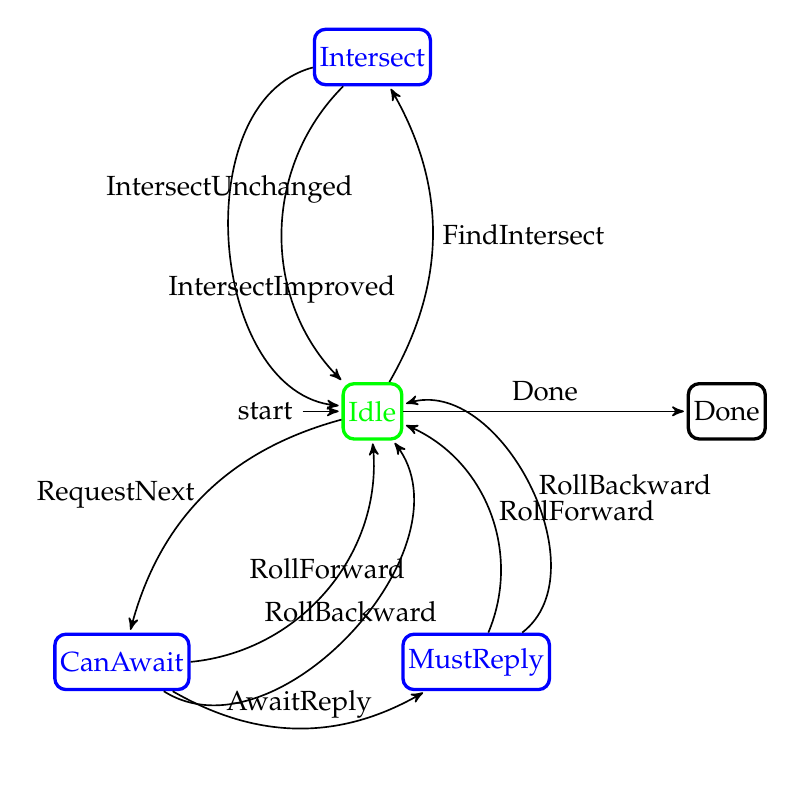
\begin{tikzpicture}[->,>=stealth',shorten >=1pt,auto,node distance=4.5cm, semithick]
  \tikzstyle{every state}=[fill=red,draw=none,text=white]
  \node[state, green, initial]                                   (Idle)      {Idle};
  \node[state, right of=Idle]                             (Done)      {Done};
  \node[state, blue, below left of=Idle]                        (CanAwait)  {CanAwait};
  \node[state, blue, right of=CanAwait]                         (MustReply) {MustReply};
  \node[state, blue, above of=Idle]                        (Intersect) {Intersect};

%  MsgRequestNext :: ChainSyncMessage header point StIdle (StNext StCanAwait)
  \draw (Idle)         edge[left, bend right]      node{RequestNext}           (CanAwait);

%  MsgAwaitReply :: ChainSyncMessage header point (StNext StCanAwait) (StNext StMustReply)
  \draw (CanAwait)     edge[above, bend right]     node{AwaitReply}            (MustReply);

%  MsgRollForward :: header -> point -> ChainSyncMessage header point (StNext any) StIdle
  \draw (CanAwait)     edge[above,bend right=45]     node{RollForward}           (Idle);
  \draw (MustReply)    edge[right,bend right=45]     node{RollForward}           (Idle);

%  MsgRollBackward :: point  -> point -> ChainSyncMessage header point (StNext any) StIdle
  \draw (CanAwait)     edge[above,bend right=80]     node{RollBackward}          (Idle);
  \draw (MustReply)    edge[right,bend right=80]     node{RollBackward}          (Idle);

%  MsgFindIntersect :: [point] -> ChainSyncMessage header point StIdle StIntersect
  \draw (Idle)         edge[right, bend right]    node{FindIntersect}         (Intersect);

%  MsgIntersectImproved  :: point -> point -> ChainSyncMessage header point StIntersect StIdle
  \draw (Intersect)    edge[above, bend right=45]    node[below = 4mm]{IntersectImproved}     (Idle);

%  MsgIntersectUnchanged :: point -> ChainSyncMessage header point StIntersect StIdle
  \draw (Intersect)    edge[above, bend right=80]    node[above = 4mm]{IntersectUnchanged}    (Idle);

%  MsgDone :: ChainSyncMessage header point StIdle StDone
  \draw (Idle)         edge[above]                node{Done}                  (Done);

\end{tikzpicture}
\end{figure}

There are to agents in the protocol: a blockchain consumer and blockchain
producer.  The protocol has two phases:
\begin{itemize}
    \item[Phase 1] In which the producer will establish a common intersection
        of consumer and producer chain;
    \item[Phase 2] In which the producer will send instructions how to
        reproduce its chain on the consumer end.
\end{itemize}
The two phases have different state machines.

\begin{figure}[H]
    \emph{Primitive types}
    \begin{equation*}
        \begin{array}{r@{~\in~}ll}
            \var{slot}                                     & \type{Slot}       & \text{slot id} \\
            \var{hash}                                     & \type{HeaderHash} & \text{hash of a block} \\
            \var{block}                                    & \type{Block}      & \text{block} \\
            \var{ReaderBackTo}\;|\;\var{ReaderForwardFrom} & \type{ReaderNext} & \text{roll-back to a reader point, or roll-forward from a reader point} \\
        \end{array}
    \end{equation*}

    \emph{Derived types}
    \begin{equation*}
        \begin{array}{r@{~\in~}ll}
            \var{point}                                  & \type{Point} = (\type{Slot}, \type{HeaderHash})                           & \\
            \var{Genesis}\;|\;\var{chain} :> \var{block} & \type{Chain}                                                              & \text{blockchain} \\
            \var{chainProducerState}                     & \type{ChainProducerState} = (\type{Chain},\type{Point},\type{ReaderNext}) & \\
        \end{array}
    \end{equation*}

    \emph{Protocol messages: Phase 1}
    \begin{equation*}
        \begin{array}{r@{~\in~}l}
            \var{MsgSetHead \var{point}}            & \var{consumer} \to \var{producer} \\
            \var{MsgIntersectImproved \var{point}}  & \var{producer} \to \var{consumer} \\
            \var{MsgIntersectUnchanged \var{point}} & \var{producer} \to \var{consumer} \\
        \end{array}
    \end{equation*}

    \emph{Protocol messages: Phase 2}
    \begin{equation*}
        \begin{array}{r@{~\in~}ll}
            \var{MsgRequestNext}               & \var{consumer} \to \var{producer} \\
            \var{MsgRollForward}\;\var{block}  & \var{producer} \to \var{consumer} \\
            \var{MsgRollBackward}\;\var{point} & \var{producer} \to \var{consumer} \\
            \var{MsgAwaitReply}                & \var{producer} \to \var{consumer} \\
        \end{array}
    \end{equation*}

    \emph{Primitive functions}
    \begin{equation*}
        \begin{array}{r@{~\in~}ll}
            \var{blockPoint} & \type{Block} \to \type{Point}                                & \\
            \var{addBlock}   & \type{Block} \to \type{Chain} \to \type{Chain}               & \text{add a block on top of a chain} \\
            \var{rollback}   & \type{Point} \to \type{Chain} \to \type{Maybe (Chain Block)} & \text{rollback a chain to a given point}  \\
        \end{array}
    \end{equation*}
\end{figure}

\subsubsection{Phase 1, establishing common intersection point}

\begin{center}
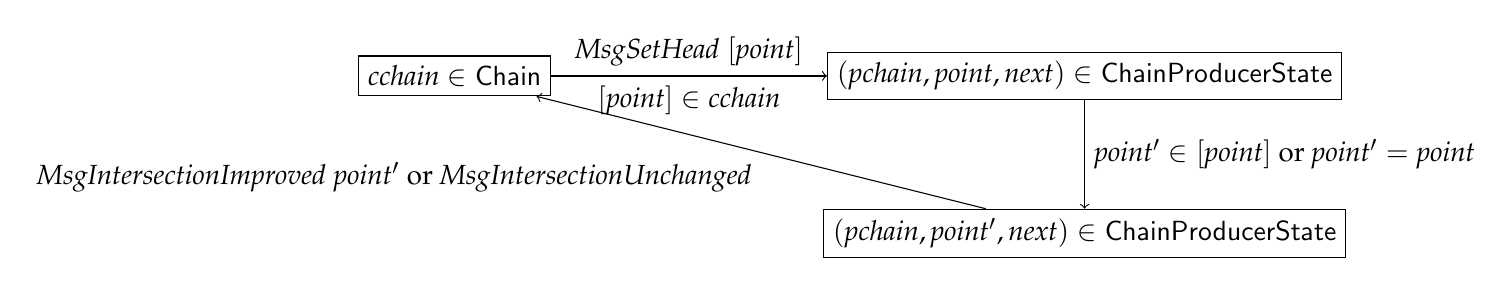
\begin{tikzpicture}
    \node (consumer1) at (0,0)   [rectangle,draw] {$\var{cchain}\in\type{Chain}$};
    \node (producer1) at (8,0)  [rectangle,draw] {$(\var{pchain}, \var{point},  \var{next})\in\type{ChainProducerState}$};
    \node (producer2) at (8,-2) [rectangle,draw] {$(\var{pchain}, \var{point'}, \var{next})\in\type{ChainProducerState}$};
    \draw[->] (consumer1) --node[above]{$\var{MsgSetHead}\;[\var{point}]$}node[below]{$[\var{point}]\in\var{cchain}$}              (producer1);
    \draw[->] (producer1) --node[right]{$\var{point'}\in[\var{point}]$ or $\var{point'} = \var{point}$}               (producer2);
    \draw[->] (producer2) --node[below left]{$\var{MsgIntersectionImproved}\;\var{point'}$ or $\var{MsgIntersectionUnchanged}$} (consumer1);
\end{tikzpicture}
\end{center}

\subsubsection{Phase 2, reproducing produer's chain on the consumer's end}

\begin{center}
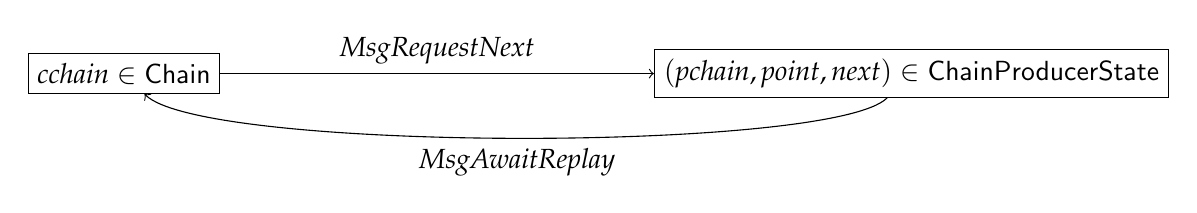
\begin{tikzpicture}
    \node (consumer1)  at (0,0)  [rectangle,draw] {$\var{cchain}\in\type{Chain}$};
    \node (producer1)  at (10,0) [rectangle,draw] {$(\var{pchain},\var{point}, \var{next})\in\type{ChainProducerState}$};
    \draw[->] (consumer1) --node[above]{$\var{MsgRequestNext}$} (producer1);
    \draw[->] (producer1) .. controls +(-1,-1) and +(1,-1) .. node[below]{$\var{MsgAwaitReplay}$} (consumer1);
\end{tikzpicture}
\end{center}

\begin{center}
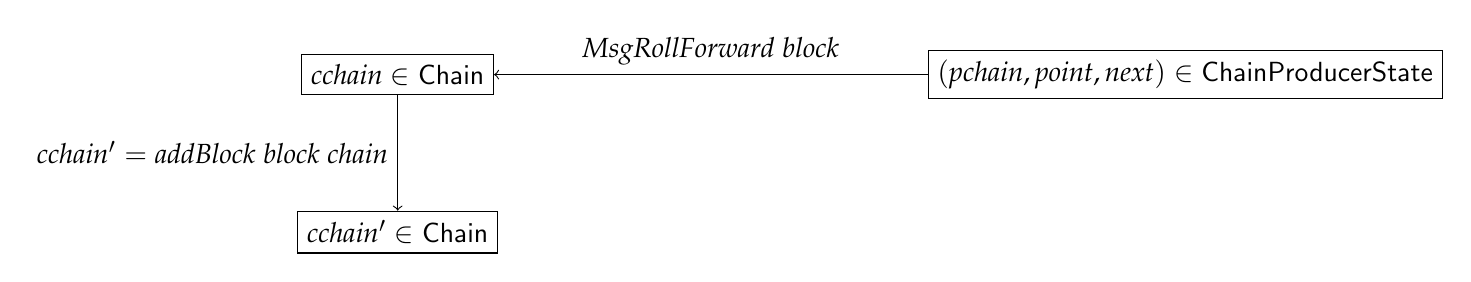
\begin{tikzpicture}
    \node (consumer1)  at (0,0)  [rectangle,draw] {$\var{cchain}\in\type{Chain}$};
    \node (producer1)  at (10,0) [rectangle,draw] {$(\var{pchain}, \var{point}, \var{next})\in\type{ChainProducerState}$};
    \node (consumer2)  at (0,-2) [rectangle,draw] {$\var{cchain'}\in\type{Chain}$};
    \draw[->] (producer1) --node[above]{$\var{MsgRollForward\;\var{block}}$} (consumer1);
    \draw[->] (consumer1) --node[left]{$\var{cchain'} = \var{addBlock}\;\var{block}\;\var{chain}$} (consumer2);
\end{tikzpicture}
\end{center}

\begin{center}
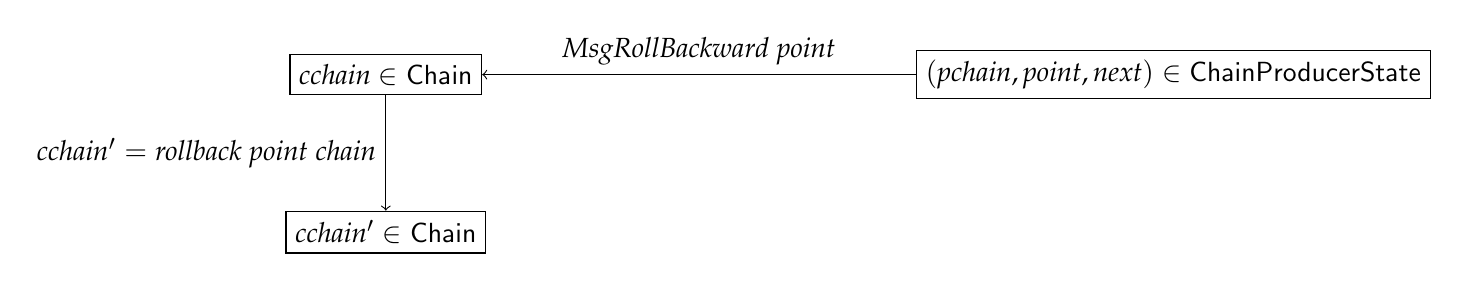
\begin{tikzpicture}
    \node (consumer1)  at (0,0)  [rectangle,draw]  {$\var{cchain}\in\type{Chain}$};
    \node (producer1)  at (10,0) [rectangle,draw]  {$(\var{pchain}, \var{point}, \var{next})\in\type{ChainProducerState}$};
    \node (consumer2)  at (0,-2)  [rectangle,draw] {$\var{cchain'}\in\type{Chain}$};
    \draw[->] (producer1) --node[above]{$\var{MsgRollBackward\;\var{point}}$} (consumer1);
    \draw[->] (consumer1) --node[left]{$\var{cchain'} = \var{rollback}\;\var{point}\;\var{chain}$} (consumer2);
\end{tikzpicture}
\end{center}

\subsubsection{Producer state transitions}
When the producer is switching a chain to another fork it needs to update its state.
\begin{center}
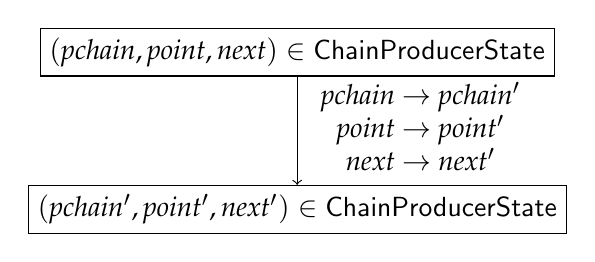
\begin{tikzpicture}
    \node (producer1)  at (0,0) [rectangle,draw]  {$(\var{pchain},  \var{point},  \var{next}) \in\type{ChainProducerState}$};
    \node (producer2)  at (0,-2) [rectangle,draw] {$(\var{pchain'}, \var{point'}, \var{next'})\in\type{ChainProducerState}$};
    \draw[->] (producer1) --node[right]{
        $\begin{array}{r@{~\to~}l}
            \var{pchain} & \var{pchain'}\\
            \var{point}  & \var{point'}\\
            \var{next}   & \var{next'}\\
        \end{array}$
    } (producer2);
\end{tikzpicture}
\end{center}
There are two cases when applying a fork.  Either 
\begin{enumerate}
    \item $\var{point}\in\var{pchain'}$, in which case $\var{next'}=\var{next}$.
    \item $\var{point}\notin\var{pchain'}$, in which case $\var{point'}=\var{intersectChains}\;\var{pchain}\;\var{pchain'}$ and $\var{next'}=\var{ReaderBackTo}$.
\end{enumerate}
After applying a fork, the producer will send to the consumer either
$\var{MsgRollForward}\;\var{block}$ or $\var{MsgRollBackward}\;\var{point'}$
according to the value of $\var{next'}$.

\bibliographystyle{apalike}
\bibliography{references}

\appendix
\section{Credible worst case scenario(s)}
\subsection{Bounding case}
\begin{itemize}
\item attacker can totally eclipse node
\item attacker has  $\rho = \frac{1}{2} - \epsilon, \epsilon > 0$ stake
\end{itemize}
\subsection{Duration of miss-information}
\begin{itemize}
\item how many slots could an attacker maintain a fiction with a)
  unfettered power of eclipse; b) $\rho$ adverserial stake at its disposal.
\item what indicators of certainty are available to inform end user?
\end{itemize}
\subsection{Inherent Assymetry}
\begin{itemize}
\item How much un-eclipsed information is needed to detect eclipse? Is
  a unicast channel enough? (this would permit other technological
  approaches in the longer run)
\item Given that a node is not totally eclipsed (i.e $\exists$
  potentially reachable non-adversrial bearer node) how does this help?
\end{itemize}  

\end{document}
